\documentclass[12pt]{report}
\usepackage{amsmath}
\usepackage{amssymb}
\usepackage{multirow}
\usepackage{graphicx}
\usepackage{tikz}
\usepackage{longtable}

\newcommand{\bt}[1]{\textbf{#1}}
\newcommand{\ubt}[1]{\textbf{\underline{#1}}}
\newcommand{\sps}{\\[0.2cm]}
\newcommand{\spn}[1]{\\[#1cm]}
\newcommand{\refn}[1]{\textbf{(\ref{#1})}}
\newcommand{\NI}{\noindent}
\newcommand{\beq}{\NI$\displaystyle}
\newcommand{\eeq}{$}
\newcommand{\eeqn}{$\\[0.3cm]}
\newcommand{\dsp}{\displaystyle}

\renewcommand*\contentsname{Table of Contents}
\renewcommand{\baselinestretch}{1.5}

\begin{document}
	\clearpage
	\thispagestyle{empty} 
	
	%%TITLE%%
	\addcontentsline{toc}{chapter}{\numberline{}Title Page}
	\begin{center}
		{\bf GENDER INEQUALITY OF CONSTRUCTION WORKERS IN TIRUCHAPPALLI (TRICHY) }
	\end{center}
	$$$$
	\begin{center}
		\textbf{\itshape\large BY}
	\end{center} 
	$$$$
	\begin{center}
		{\bf ABDULKAREEM, Lawal Babaita\\
			16/30GP002}
	\end{center}
	$$$$
	\begin{center}
		\textbf{A PROJECT SUBMITTED TO THE
			DEPARTMENT OF MATHEMATICS, FACULTY OF PHYSICAL SCIENCES,
			UNIVERSITY OF ILORIN, ILORIN, NIGERIA,
			$$$$
			IN PARTIAL 
			FULFILLMENT OF REQUIREMENTS FOR THE AWARD OF
			BACHELOR OF SCIENCE {\itshape{(B.Sc.)}} DEGREE IN MATHEMATICS.}
	\end{center}
	$$ $$ 
	\\ \\
	\begin{center}
		{\bf 	JUNE, 2021}
	\end{center}
	%%%%CERTIFICATION%%%%%
	\newpage
	\pagenumbering{roman}
	\addcontentsline{toc}{chapter}{\numberline{}Certification}
	\section*{\begin{center}\textbf{\Large Certification}   \end{center}}
	This is to certify that this project was carried out by \textbf{ABDULKAREEM, Lawal Babaita} of Matriculation Number  16/30GP002, for the award of Bachelor of Science B.Sc (Hons) degree in the Department of Mathematics, Faculty of Physical sciences, University of Ilorin, Ilorin, Nigeria.
	\\
	\\
	................................... \qquad \qquad\qquad\qquad\qquad\qquad...................... \\
	PROF. K. RAUF   ~~\qquad\qquad\qquad\qquad\qquad\qquad\qquad\quad Date\\
	(SUPERVISOR)\\
	\\
	\\
	\\
	...................................... \qquad\qquad\qquad\qquad\qquad\qquad ......................\\
	PROF. K. RAUF      \qquad\qquad\qquad\qquad\qquad\qquad\qquad\qquad     Date\\
	(HEAD OF DEPARTMENT)\\
	\\
	\\
	\\
	..................................... \qquad\qquad\qquad\qquad\qquad\qquad .......................\\
	PROF. T. O. OLUYO  \qquad\qquad\qquad\qquad\qquad\qquad \quad~        Date\\
	(EXTERNAL EXAMINER)
	
	\newpage
	%%DEDICATION%%
	\section*{\begin{center}	\textbf{\Large Dedication}   \end{center}}
	\addcontentsline{toc}{chapter}{\numberline{}Dedication}
	
	This project work is dedicated to Almighty Allah uncreated creator and my entire family.
	
	\newpage
	%%ACKNOLEDGEMENT%%
	\section*{\begin{center}\textbf{\Large Acknowledgments}\end{center}}
	\addcontentsline{toc}{chapter}{\numberline{}Acknowledgments} 					
	The effort of the non-academic staff of the department are equally appreciated.
I give all glory, honor and reverence to God Almighty for the exceeding grace and love that He bestowed on me and sustaining me in my journey, and also for ability to write this project.
I appreciate my supervisor Prof. K. Rauf for his fatherly support towards this work. God bless and your family sir.
And I also want to acknowledge my level adviser, Dr(Mrs) I. F. Usamot,for her encouraging words, concern and guidance.
A well honouring gratitude toProfessors J. A Gbadeyan,  T. O. Opoola,  O. M. Bamigbola,  M. O. Ibrahim,  O. A. Taiwo,  R. B. Adeniyi,  K. O. Babalola, M.S. Dada,  A. S. Idowu and  Doctors E. O. Titiloye, Mrs.Y.O. Aderinto, Mrs. C. N. Ejieji,  B.M. Yisa, J.U. Abubakar, K .O. Bello, Mrs. G. N. Bakare, B.M. Ahmed,  O. T. Olotu,  A. O. Uwaheren , O. Odetunde, T.L. Oyekunle, A.A. Yeketi and other staffs of the department of Mathematics.
I also want to Acknowledge my parents for their love and support in this project.
	
	\newpage
	%%ABSTRACT%%
	\section*{\begin{center}\textbf{\Large Abstract}\end{center}}
		\addcontentsline{toc}{chapter}{\numberline{}Abstract}
		Gender inequality plays an important role in establishing the description and quantifying the distribution of certain variables in the study of of population at one point of time, and cover the following socio-economic ethics of men construction workers, the reasons for involving women in mansory.
		
	%%TABLE OF CONTENTS%%
	\addcontentsline{toc}{chapter}{\numberline{}Table of Contents}
	\tableofcontents
	\newpage
	
	\pagenumbering{arabic}
	%%%%%%%%%%%%%%%%%%%%%%%%%CHAPTER ONE%%%%%%%%%%%%%%%%%%%%%%%%%%%%
	\chapter{}
	\section{INTRODUCTION TO INEQUALITIES}
	Mathematicians as well as Mathematics educators can attest to the importance of inequalities not only in the study of Mathematics but also n the normal life activities.
	
	Consider building blocks for many Mathematical areas, inequalities are studied for three particular reasons, which are as follows;
	\begin{itemize}
		\item Practical
		\item Theoretical and
		\item Aesthetic
	\end{itemize}

	\subsection{PRACTICAL}
	At the practical level, from the early involvement with problem solving, one must learn to build variables or learn to write restrictions for the unknowns, and these are expressed as inequalities.
	
	\subsection{THEORETICAL}
	Theoretically, inequalities used to express the domain of a function to prove limits, to setup research questions that relate equations to special cases that are inequalities or to prove equality by means of inequalities.\spn{-.3}
	
	\NI Moreover, Mathematicians testify that there are many aesthetic aspects in inequalities as well as in some of their proofs.
	
	\subsection{AESTHETIC}
	Aesthetic in Mathematics encompasses an appreciation of the beauty elegance and significance of Mathematical entities. A generation of hormonions and permanent patterns, a perseverance in continuing a journey even when one is lost in misleading positions. All these aspects are present in the work of a Mathematicians concerned with inequalities.
	
	
	\section{DEFINITION OF INEQUALITIES}
	\begin{description}
		\item[DEF 1.1] Inequalities is comparison of two values or expressions. An inequalities compares two statements with different values.
		\item[DEF 1.2] In Mathematics, Inequalities is a relationship between two different quantities or values.
	\end{description}
	Inequalities is a Mathematical expression that one quantity is greater than or less than another quantity.
	
	\NI\bt{For Example}\\
	"a\bt{ is less than } b"\spn{-.4}
	
	\NI \bt{NOTE:} The above expression can be written symbolically\\
	$\displaystyle a < b$ [i.e the left hand side is lower than \{ i.e less than\} the right hand side]\spn{-0.3}
	
	\NI Also,\\
	"a \bt{is greater than } b"\\
	It can also be written symbolically as,\\
	$\displaystyle a > b$ [i.e the left hand side is greater than \{ i.e higher than\} the right hand side]\spn{-0.3}
	
	\NI The above expressions are examples of inequalities.\\
	
	\NI Also, the express $x$ greater than 10 \{i.e symbolically $x > 10$ \} is an inequality, whereas, $x$ equal to 10 \{ i.e symbolically $x = 10$ \} is an equation.\\
	
	\NI Recall that an equation is a statement declaring the equality of two expressions.
	
	\NI For example; $5x + 5 = 3$ is an equation\spn{-.5}
	
	\NI And inequality compares two statements with different values. Example $5x + 5 \leq 30$ is an inequality.
	
	\section{THE USE OF SYMBOLS IN INEQUALITIES}
	
	The use of symbols make inequalities expression in Mathematics more easier to express.\spn{-.3}
	
	\NI The inequality expression "a is less than b" is easily denoted by "$a < b$", also the inequality expression "a is greater than b" is easily denoted by "$a > b$".\spn{-.4}
	
	\NI Also, we can also have the inequality expression "a is greater than or equal to b" and "a is less than or equal to b" which is also symbolically denoted by "$a \geq b$" and "$a \leq b$" respectively.\spn{-.3}
	
	\NI Therefore, we can easily say inequalities is defined whenever we have two expressions linked with one of the following five(5) symbols
	\begin{enumerate}
		\item $<$ \quad ---\quad less than \{the left hand side is less than the right hand side\}
		
		\item $>$ \quad ---\quad greater than \{the left hand side is greater than the right hand side \}
		
		\item $\leq$ \quad ---\quad less than or equal to \{the left hand side is less than or equal to the right hand side \}
		
		\item $\geq$ \quad ---\quad greater than or equal to \{the left hand side is greater than or equal to the right hand side\}
		
		\item $\neq$ \quad ---\quad not equal to \{the left hand side is not equal to the right hand side\}
	\end{enumerate}
	\section{RULES FOR INEQUALITIES}
	\begin{enumerate}
		\item $A\leq B \implies A + C \leq B + C$
		\item $A \leq B \implies A - C \leq B - C$
		\item if $C > 0$, then $A \leq B \implies CA \leq CB$
		\item if $C < 0$, then $A \leq B \implies CA \geq CB$
		\item if $A > 0$ and $B > 0$, then $A \leq B \implies \frac{1}{A} \geq \frac{1}{B}$
		\item if $A \leq B$ and $C \leq D$, then $A + C \leq B + D$
	\end{enumerate}
	
	\section{NOTATIONS IN INEQUALITIES}
	\begin{enumerate}
		\item $a<b$ (means $a$ is smaller than $b$)
		\item $a>b$ (means $a$ is greater than $b$)
		\item $a \leq b$ (means $a$ is smaller/less than or equal to $b$)
		\item $a \geq b$ (means $a$ is greater than or equal to $b$)
		\item $a \neq b$ (means $a$ is not equal to $b$)
	\end{enumerate}
		
	\section{TYPES OF INEQUALITIES}
	\begin{enumerate}
		\item LINEAR INEQUALITIES
		\item QUADRATIC INEQUALITIES
		\item COMPOUND INEQUALITIES
		\item ABSOLUTE VALUE INEQUALITIES
	\end{enumerate}
		
	\subsection{LINEAR INEQUALITIES}
	A Linear inequality is an inequality which involves a linear function. A linear inequality looks exactly like a linear equation with the inequality sign replacing the equality sign.\\
		
	\NI \ubt{Examples of Linear Inequalities}
	\begin{enumerate}
		\item $x^2 + 5x \leq 22$ (i.e $x^2 + 5x$ is less than or equal to 22)
			
		\item $5x + 7 < 7$ (i.e $5x + 7$ is less than 7)
			
		\item $7y^2 - 4 \geq 6$ (i.e $7y^2 - 4$ is greater than or equal to 6)
			
		\item $4x + 14 > 10$ (i.e $4x + 14$ is greater than 10)
			
		\item $2x^3 - 4 \neq 5$ (i.e $2x^3 - 4$ is not equal to 5)
	\end{enumerate}
	
	\subsection{QUADRATIC INEQUALITIES}
	A quadratic inequalities is a function whose degree is 2 and where the $y$ is not always exactly equal to the function. These types of functions use symbols called inequality symbols that include the symbols we known \bt{"less than, greater than, less than or equal to and greater than or equal to}. So instead of seeing an equal sign, you will see these inequality symbols.\\
		
	\NI All quadratic inequalities are of the form $\mathbf{ax^2 + bx + c}$, where $\mathbf{a}$, $\mathbf{b}$ and $\mathbf{c}$ are numbers. The numbers $\mathbf{b}$ and $\mathbf{c}$ can be $\mathbf{0}$, but $\mathbf{a}$ must be equal to a number. It cannot be $\mathbf{0}$. This is because our quadratic inequality must have an $\mathbf{x^2}$ value. The other two terms do not need to be there.\\
		
	\NI\ubt{Examples}
	\begin{enumerate}
		\item $x^2 + 5x \leq 10$ (i.e $x^2 + 5x$ is less than or equal to 10)
			
		\item $x^2 + 2x \geq 5$ (i.e $x^2 + 2x$ is greater than or equal to 5)
	\end{enumerate}
	
	\subsection{COMPOUND INEQUALITIES}
	A compound inequalities is an equation with two or more inequalities joined together with either \bt{"and"} or \bt{"Or"}\\
		
	\NI\ubt{Examples}
	\begin{enumerate}
		\item $x \geq b$ and $x < 3$
		\item $x < -12$ or $x \geq 8$
	\end{enumerate}
		
	When two inequalities are joined with \bt{"and"}, they are often written simply as a double inequality, for example $-6 \leq x < 3$. The solution of an \bt{"and"} in inequalities is the intersection of each individual inequality in the sentence.
		
	\subsection{ABSOLUTE VALUE INEQUALITIES}
	Let first return to the original definition of absolute value;\\
	
	\NI Absolute Value $(x)$ is the distance of $x$ from zero. For instance, both $-2$ and $+2$ are two units from zero, as it is shown in the image below\\
		
	\begin{center}
		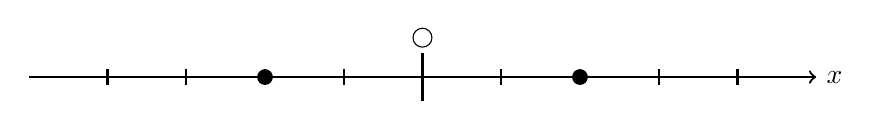
\begin{tikzpicture}
			\draw[thick, ->] (-1,0) -- (9,0) node[right]{$x$};
			\foreach \x in {0,1,...,8}
				\draw[thick] (\x,0.1) -- (\x,-0.1);
			\draw[thick] (4,.3) -- (4,-.3);
			\draw (4,.5) circle(1.2mm);
			\fill (2,0) circle(1mm);
			\fill (6,0) circle(1mm);
		\end{tikzpicture}
	\end{center}
		
	\NI This means that these absolute values will both be 2: that is, we have $|-2| = |+2| = 2$\\
	
	\NI With this definition and image in mind, let's now define Absolute Value Inequalities.\spn{-.5}
		
	\NI\bt{Absolute Value Inequality is an inequality that has an absolute value sign with a variable inside.}\spn{-.4}
		
	\NI\ubt{Examples}\\
	$|x| < 4$ (means that the distance between $x$ and $0$ is less than $4$)\\
	$|x| > 3$ (means that the distance between $x$ and $0$ is greater than $3$)\\
		
	\subsubsection{PROPERTIES OF AN ABSOLUTE VALUE INEQUALITIES}
	\begin{enumerate}
		\item $|x| < C \implies -C < x < C$ (i.e the distance between $0$ and $x$ is less than $C$)
			
		\item $|x| \leq C \implies -C \leq x \leq C$ (i.e the distance between $0$ and $x$ is less than or equal to $C$)
			
		\item $|x| > C \implies -C > x > C$ (i.e the distance between $0$ and $x$ is greater than $C$)
			
		\item $|x| \geq C \implies -C \geq x \geq C$ (i.e the distance between $0$ and $x$ is greater than or equal to $C$)
	\end{enumerate}
	
	\section{EXAMPLES OF INEQUALITIES IN DAILY LIFE}
	\NI(1) If Ade has N100 and wants to buy some biros and pencils, how many biros and pencils can he buy? Using inequality expression, write this statement Mathematically.\spn{-.6}
		
	\NI\ubt{Solution}\\
	Let number of biros be $x$\\
	and let number of pencils be $y$\\
	Amount owned by Ade $= \text{N}100$\\
	Therefore; $x + y \leq 100$\\
		
	\NI(2) Ibrahim receives N200 daily for his daily needs if he need to buys some books and bottle of water, how many books and bottle of water can he buy using inequality expression, thus, write this statement Mathematically\spn{-.6}
		
	\NI\ubt{Solution}\\
	Amount owned by Ibrahim $=\text{N}200$\\
	Let number of books bought be $=a$\\
	and let number of bottle of water bought be $=b$\\
	Therefore, $200 \geq a+b$\\
		
	\NI(3) Ola is a father of three children (Ade, Ope, and Tade). If the ages of the three children is added together and subtracted from Ola's age. How old is Ola. Use the inequality expression and write this statement Mathematically.\spn{-.6}
		
	\NI\ubt{Solution}\\
	Let Ola's age be $Q$\\
	Let the ages of Ola's children (Ade, Ope and Tade) be $x, y, z$ respectively,\\
	Therefore; $x + y + z \geq Q$\\
	
	
	
	%%%%%%%%%%%%%%%%%%%%%%%%%CHAPTER TWO%%%%%%%%%%%%%%%%%%%%%%%%%%%%
	\chapter{PROPERTIES OF INEQUALITIES}
	
	\subsubsection{(1) TRANSITIVE PROPERTY}
	The transitive property of inequality state that, for any real number $a,b,c,$
	\begin{enumerate}
		\item if $a > b$ and $b>c$, then $a > c$ (if $a$ is greater than $b$ and $b$ is greater than $c$, then $a$ is greater than $c$)
		
		\item if $a>b$ and $b \geq c$, then $a>c$ (if $a$ is greater than $b$ and $b$ is greater than or equal to $c$, then $a$ is greater than $c$)
		
		\item if $a < b$ and $b<c$, then $a<c$ (if $a$ is less than $b$ and $b$ is less than $c$, then $a$ is less than $c$)
	\end{enumerate}
	\newpage
	\ubt{Example}\\
	(1)If Ola is older than Ore and Ope is older than Tola, then Ola is older than Tola\\
	(2) If Tola has 4 mangoes and Ope has 3 mangoes, but Ola has 1 mango,\\
	Let represent mangoes owned by Tola to be $X$\\
	Let represent mangoes owned by Ope to be $Y$\\
	and, let represent mangoes owned by Ola to be $Z$\\
	then, $X>Y, \quad Y>Z, \text{ then } X >Z$\\
	
	\subsubsection{(2) REVERSAL PROPERTY}
	The Reversal property of inequality states that; for any real value $a$ and $b$,\\
	(1) if $a$ is greater than $b$, the $b$ is less than $a$. i.e if $a>b$, then $b<a$\\
	\ubt{Example}\\
	If Ola is older than Ope, then Ope is younger than Ola.
	
	\subsubsection{(3) LAW OF TRICHOTOMY}
	The law of trichotomy states that only one of the following is true: $a<b$, or $a=b$, or $a>b$\\
	
	\NI\ubt{Example}\\
	If Ola has more money than Ope, then we could write it like $a>b$ (representing Ola and Ope with $a$ and $b$ respectively)\\
	Also, we know that\\
	
	\NI Ola does not have less money than Ope (Not $a<b$)\\
	And, Ola does not have equal or the same money as Ope (Not $a \neq b$)
	
	\subsubsection{(4) SQUARE ROOT PROPERTY}
	It says taking a square root will not change the inequality but only when both $a$ and $b$ are greater than or equal to zero. That is, if $a<b$ then $\sqrt{a} \leq \sqrt{b}$ (for $a,b\geq 0$)\\
	
	\NI The above expression means if $a$ is less than or equal to $b$, then $\sqrt{a}$ is less than or equal to $\sqrt{b}$, if $a$, $b$ is greater than or equal to zero.\\
	
	\NI\ubt{Example}\\
	Let $a=4$\quad and\quad $b=25$\\
	So, if $a\leq b$\quad is\quad $4\leq 25$\\
	then $\sqrt{a} \leq \sqrt{b}$\quad is\quad $\sqrt{4} \leq \sqrt{25}$ (for $a,b \geq0$)
	
	\subsubsection{(5) ADDITION AND SUBTRACTION}
	It says that a common constant $c$ may be added or subtracted from both side of an inequality.\\
	That is, if $a<b$, then $a+c < b + c$\\
	
	\NI Also, for any real numbers $a, b, c$
	\begin{enumerate}
		\item if $a\leq b$, then $a+c \leq b+c$ and $a-c \leq b-c$
		
		\item if $a\geq b$, then $a+c \geq b+c$ and $a-c \geq b-c$
	\end{enumerate}
	
	\subsubsection{(6) ADDITIVE INVERSE}
	The Additive Inverse property states that; for any real numbers $a$ and $b$, negation will invert the inequality use
	\begin{enumerate}
		\item if $a \leq b$, then $-a \geq -b$
		
		\item if $a>b$, then $-a < -b$
	\end{enumerate}
	
	\NI As we just away, putting minuses(-) in from of real numbers $a$ and $b$ changes the direction of the inequality.\spn{0.3}
	This is called the Additive Inverse
	\begin{itemize}
		\item if $a<b$, then $-a > -b$
		\item if $a>b$, then $-a < -b$
	\end{itemize}
	
	\NI This is really the same as multiplying by (-1), and that is why it changes direction
	
	\subsubsection{(7) MULTIPLICATIVE INVERSE}
	The property for the multiplication inverse state that; for any non-zero real number $a$ and $b$, that are both positive or both negative, taking the reciprocal $\left(\text{i.e } \frac{1}{\text{value}}\right)$ of both $a$ and $b$ can change the direction of the inequality.\\
	
	\NI When $a$ and $b$ are both positive or both negative, i.e;
	\begin{itemize}
		\item if $a<b$ then $\frac{1}{a} > \frac{1}{b}$
		\item if $a>b$ then $\frac{1}{a} < \frac{1}{b}$
	\end{itemize}
	
	\NI These can also be written in chained notation as follows:\\
	for any non-zero real numbers $a$ and $b$;
	\begin{enumerate}
		\item if $0<a \leq b$, then $\frac{1}{a} \geq \frac{1}{b} > 0$
		\item if $a<b<0$, then $0 > \frac{1}{b} > \frac{1}{a}$
		\item if $a<0<b$, then $\frac{1}{a}<0<\frac{1}{b}$
		\item if $0\geq0>b$, then $\frac{1}{b} < \frac{1}{a} \leq 0$
		\item if $a>b>0$, then $0 < \frac{1}{b} < \frac{1}{a}$
	\end{enumerate}	
	
	\section{POWER INEQUALITIES}
	A Power Inequality is an inequality containing terms of the form $a^b$, where $a$ and $b$ are real positive numbers or variable expressions.\spn{0.4}
	\ubt{Examples}\\
	for any real number $x$,
	\begin{enumerate}
		\item $e^x \geq 1 + x$
		\item if $\displaystyle x>0$ and $p>0$, then \\ $\frac{x^p-1}{p} \geq \ln(x) \geq \frac{1-\frac{1}{x^p}}{p}$ \\
		
		\NI In the limit of $p\rightarrow 0$, then upper and lower bounds converge to $ln(x)$
		
		\item if $x>0$, then \\
		     $\displaystyle x^x \geq (\frac{1}{e})^{\frac{1}{e}}$
		
		\item $x \geq 1$, then\\
			$\dsp (x+y)^z + (x+z)^z + (y+z)^x > 2$
			
		\item for any real distinct numbers $a$ and $b$\\
			$\dsp \frac{e^b - e^a}{b-a} > e^{(a+b)/2}$
	\end{enumerate}
	
	\section{THE NUMBER LINE}
	a number line is a line with numbers on it i.e
	\begin{center}
		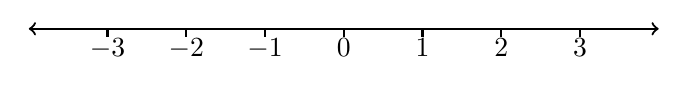
\begin{tikzpicture}
			\draw[thick, <->] (-4,0) -- (4,0);
			\foreach \x in {-3,-2,...,3}
			\draw[thick] (\x,-0.1)--(\x,0) node[below]{$\x$};
		\end{tikzpicture}
	\end{center}
	We use a number line to count and to graphically show numbers\\
	\ubt{Example}\\
	\begin{enumerate}
		\item Graph $x=5$ is expressed as\\
		\begin{center}
			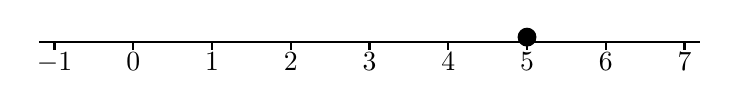
\begin{tikzpicture}
				\draw[thick] (-1.2,0) -- (7.2,0);
				\fill (5,0.06) circle(1.2mm);
				\foreach \x in {-1,0,...,7}
					\draw[thick] (\x,-0.1)--(\x,0) node[below]{$\x$};
			\end{tikzpicture}
		\end{center}
	
		\item Graph $x=-4$ is expressed as\\
		\begin{center}
			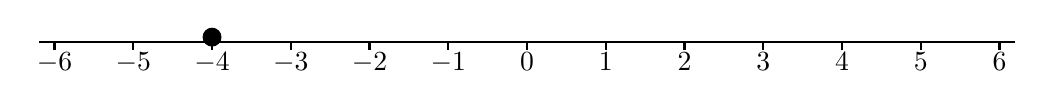
\begin{tikzpicture}
				\draw[thick] (-6.2,0) -- (6.2,0);
				\fill (-4,0.06) circle(1.2mm);
				\foreach \x in {-6,-5,...,6}
				\draw[thick] (\x,-0.1)--(\x,0) node[below]{$\x$};
			\end{tikzpicture}
		\end{center}
	\end{enumerate}
	\newpage
	\section{GRAPHING INEQUALITIES}
	Graph $x<3$
	\begin{center}
		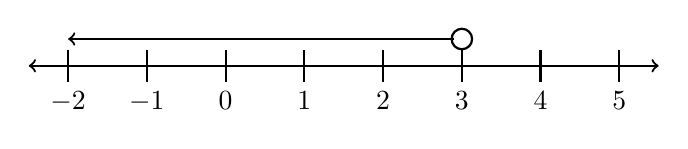
\begin{tikzpicture}
			\draw[thick, <->] (-2.5,0) -- (5.5,0);
			\draw[thick, <-] (-2,0.34) -- (2.9,0.34);
			\draw[thick] (3,0.34) circle(1.3mm);
			\foreach \x in {-2,-1,...,5}
				\draw[thick] (\x,0.2)--(\x,-0.2) node[below]{$\x$};
		\end{tikzpicture}
	\end{center}
	Also, Graph $x\leq3$
	\begin{center}
		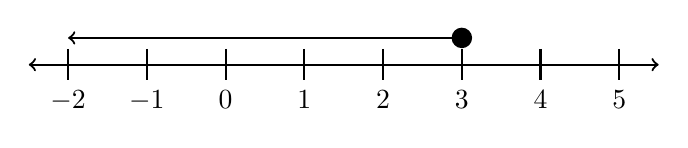
\begin{tikzpicture}
			\draw[thick, <->] (-2.5,0) -- (5.5,0);
			\draw[thick, <-] (-2,0.34) -- (2.9,0.34);
			\fill (3,0.34) circle(1.3mm);
			\foreach \x in {-2,-1,...,5}
			\draw[thick] (\x,0.2)--(\x,-0.2) node[below]{$\x$};
		\end{tikzpicture}
	\end{center}
	\bt{Note:}
	\begin{itemize}
		\item The solid shows that range of value that $x$ can take.
		\item The open circle on $3$ shows that although the solid line goes from 3, but $x$ cannot actually be equal to 3.
		\item The painted circle shows that $x$ can either be less than or equal to 3.
	\end{itemize}
	
	\NI\ubt{Examples}\\
	(1) Solve the inequality $4x + 6 > 3x + 7$ and represent the result on a number line\\
	\ubt{Solution}
	$4x + 6 > 3x + 7$\\
	firstly, we subtract 6 from both sides:\\
	we get; \quad $4x + 6-6 > 3x + 7 - 6$\\
	  $\left.\right.$\quad\qquad\quad= $4x > 3x + 1$\\
	Now, we subtract $3x$ from both sides\\
	We get, \quad $4x - 3x > 3x - 3x + 1$\\
	$\left.\right.$\quad\qquad\quad = $x > 1$\\
	representing $x>1$ on a number line\\
	\begin{center}
		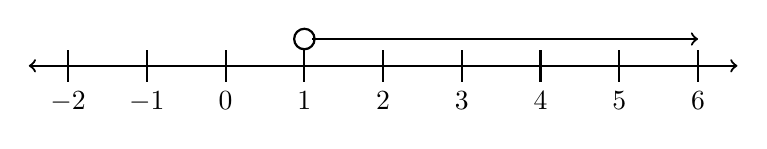
\begin{tikzpicture}
			\draw[thick, <->] (-2.5,0) -- (6.5,0);
			\draw[thick, ->] (1.1,0.34) -- (6,0.34);
			\draw[thick] (1,0.34) circle(1.3mm);
			\foreach \x in {-2,-1,...,6}
			\draw[thick] (\x,0.2)--(\x,-0.2) node[below]{$\x$};
		\end{tikzpicture}
	\end{center}

	\NI(2) For what values of $x$ are both the inequalities $9+2x >0$ and $7-3x>0$ are true?\\
	\ubt{Solution}\\
	if $9 + 2x>0$\\
	subtracting 9 from both sides,\\
	we get; \quad $9+2x-9>0-9$\\
	$\left.\right.\qquad\qquad 9-9 + 2x > 0-9$\\
	$\left.\right.\qquad\qquad = 2x > 0-9$\\
	$\left.\right.\qquad\qquad = 2x > -9$ 0r $\dsp x> -\frac{9}{2}$\\
	
	\NI Also, if $7-3x > 0$\\
	Subtracting $7$ from both sides\\
	We get; \quad $7-3x-7> 0 -7$\\
	$\left.\right.\qquad\qquad -3x > -7$ (negative cancels negative)\\
	$\left.\right.\qquad\qquad \implies 3x < 7$ or $\dsp x < \frac{7}{3}$\\
	
	\NI (Note: the reversed of the sign occurs when we divided both of the inequality by a negative numbers)\\
	We see that both sides inequalities are true for\\
	$$-\frac{9}{2} < x < \frac{7}{3}$$

	\NI representing the above inequality expression on a number line, we have;\\
	\begin{center}
		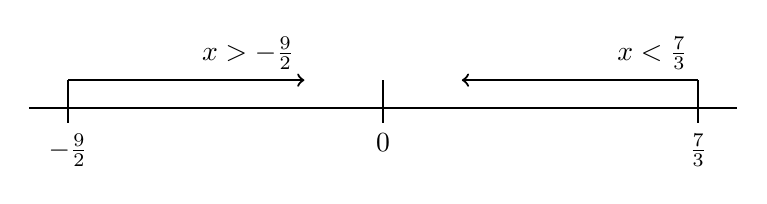
\begin{tikzpicture}
			\draw[thick] (-0.5,0)--(8.5,0);
			\draw[thick, ->] (0,0.35) -- (3,0.35) node[above left]{$x > -\frac{9}{2}$};
			\draw[thick, <-] (5,0.35) -- (8,0.35) node[above left]{$x < \frac{7}{3}$};
			\foreach \x /\y in{0/$-\frac{9}{2}$,4/0,8/$\frac{7}{3}$}
				\draw[thick] (\x,0.35)--(\x,-0.2) node[below]{\y};
		\end{tikzpicture}
	\end{center}
	
	\section{INEQUALITIES USED WITH A MODULUS SYMBOL}
	Inequalities often appear in conjunction with the modulus, or absolute value symbol $"|\;\;|"$ e.g $|x|<2$\\
	
	\NI Recall that the modulus of a number is simply its magnitude, or absolute value, regardless of its signs. So,\\
		$\left.\right.\qquad\qquad\qquad\qquad\qquad\qquad$ $|2|=2$ and $|-2|=2$\\
		
	\NI Now, $|x|<2$, it implies that $x$ must lies between 2 and -2, we can write it as $-2<x<2$, the range of value is shown in the number line, as shown below;
	\begin{center}
		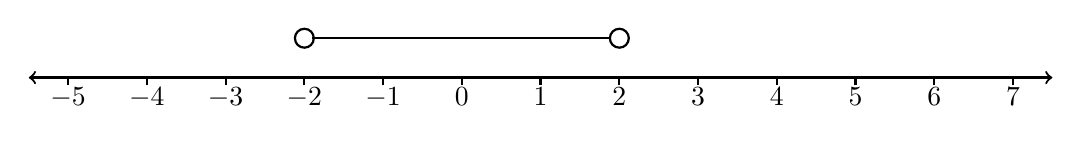
\begin{tikzpicture}
			\draw[thick, <->] (-5.5,0) -- (7.5,0);
			\draw[thick] (-2,0.5) circle(1.2mm);
			\draw[thick] (2,0.5) circle(1.2mm);
			\draw[thick] (-1.9,0.5) -- (1.9,0.5);
			\foreach \x in {-5,-4,...,7}
				\draw[thick] (\x,-0.1)--(\x,0) node[below]{$\x$};
		\end{tikzpicture}
		A number line showing $-2 < x < 2$\\
	\end{center}
	\ubt{Example}\\
	Suppose we want to solve the inequality $|x|\geq 5$\\
	
	\NI\ubt{Solution}\\
	If $|x| \geq 5$; This mean that the absolute value of $x$ must be greater than or equal to 5.\\
	
	\NI This also means that $x$ can be greater than or equal 5, or can be less than or equal to -5, we write $x\leq -5$ or $x\geq 5$. The range of values is shown below;
	\begin{center}
		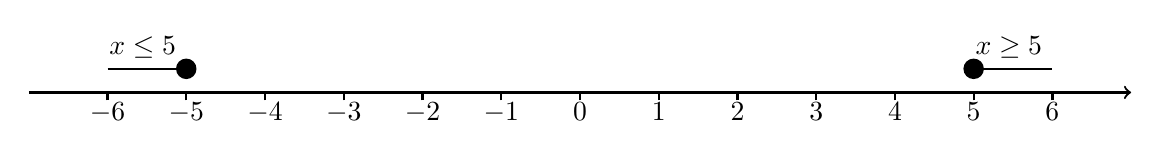
\begin{tikzpicture}
			\draw[thick,->](-7,0) -- (7,0);
			\draw[thick] (-6,0.3) -- (-5,0.3) node[above left]{$x\leq 5$};
			\draw[thick] (5,0.3) -- (6,0.3)node[above left]{$x\geq 5$};
			\fill (-5,0.3) circle(1.3mm);
			\fill (5,0.3) circle(1.3mm);
			\foreach \x in {-6,-5,...,6}
				\draw[thick] (\x,-0.1)--(\x,0) node[below]{$\x$};
		\end{tikzpicture}
		A number line showing $|x| \geq 5$\\
	\end{center}
	
	
	%%%%%%%%%%%%%%%%%%%%%%%%%CHAPTER THREE%%%%%%%%%%%%%%%%%%%%%%%%%%%%
	\chapter{RESEARCH METHODOLOGY}
	
	Objectives  of  study The  objectives  of  the  study  are  to  find  out  the  reasons  why  women  construction workers  should  be  empowered  to  become  masons,  to  determine  the  process  by  which men  are  being  trained  in  construction  sector,  to  determine  the  willingness  of  women construction  workers  to  become  masons  and  the  willingness  of  men  construction  workers and  contractors  to  train  and  employ  women  as  masons.  There  are  many  studies  on construction  sector  which  recommend  that  women  could  be  empowered  by  training  to  do the  tasks  of  masons  in  India  (Habitat,  1997;  ILO,  2001;  Baruah,  2008).\\
	
	But  there  is hardly  any  study  in  India  which  identifies  the  barriers  which  prevent  women  construction workers  from  undertaking  masonry  work  and  the  process  by  which  these  women  could  be empowered  in  the  construction  sector.  This  study  is  again  an  attempt  to  determine  the 5Women have  only  one  job  title  chithal,  which  means  one  who  is  small  in  the  local  language.  Women  enter as  chithal  and  retire  as  chithal  and  they  also  receive  the  wages  of  chithal,  which  remains  the  same.  Men have  many  job  titles  like  centering  laborers,  periyal  (one  who  is  big),  manvettial  (one  who  digs),  masons, supervisors  and  contractors.  Thus  men  can  be  promoted  to  masons, supervisors  and  finally  contractors,  whereas  women  have  no  scope  for  promotion. Which  prevent  women  construction  workers  from  being  promoted  as  masons  and find  out  a  methodology  for  training  women  construction  workers  in  Tamil  Nadu  (India). 
	
	
	\section{AREA OF STUDY}
	This  is  a  descriptive  study  conducted  in  the  Indian  state  of  Tamil Nadu.  Tamil Nadu  is  located  in  the  southernmost  tip  of  the  Indian  Peninsula  bordered  by  Kerala  to  the west,  Karnataka  to  the  northwest,  Andhra  Pradesh  to  the  north  and  Bay  of  Bengal  to  the east  (Pan  India  Networks,  2009a).  The  total  area  covered  by  the  state  is  130,058  sq.  kms. According  to  the  Indian  Census  (2001),  Tamilnadu  has  a  total  population  of  62,405,679.\\
	
	Tiruchirapalli  District  is  located  along  banks  of  the  River  Kaveri  in  Tamil  Nadu  state  of India  (Pan  India  Networks,  2009b).  Trichy  is  a  municipal  corporation  and  the administrative  headquarters  of  Tiruchirapalli  District.  Tiruchirapalli,  has  a  population  of 2,418,366  (Census  of  India,  2001).  Males  constitute  49.97  per  cent  of  the  population  and females  50.03  per  cent.  The  total  number  of  workers  are  1,064,521,  they  constitute 687,814  male  workers  (64.6  per  cent)  and  376,707  female  workers  (35.4  per  cent). 
	
	
	\section{DATA COLLECTION METHOD AND TOOLS}
	 In  this  study,  stratified  sampling  was  used.  A  sample  of  440  women  construction workers  in  Tiruchirapalli  district  was  interviewed  to  find  out  their  views  on  women  in masonry  and  their  skills  to  be  trained  as  women  masons.  A  sample  of  440  men construction  workers  in  Tiruchirapalli  district  was  interviewed  to  find  out  the  way  in which  they  are  trained  for  masonry  work.  A  sample  of  51  Contractors/  Engineers  in Tiruchirapalli  district  was  asked  to  fill  questionnaire  to  find  out  their  views  on  women  in masonry  work  in  construction  sector.    The  construction  workers  were  selected  from Santhai  (place  where  they  are  recruited  for  work),  workplaces  and  wage  disbursement centers.\\
	 
	 The  Primary  data  collected,  is  through  interview  schedule.  As  majority  of  the construction  workers  are  illiterate,  two  schedules  were  prepared,  one  for  women construction  workers  and  another  for  men  construction  workers,  and  the  construction workers  were  interviewed  in  the  local  language  (Tamil)  and  the  responses  were  noted  in the  schedule.     
	
	
	
	\section{FINDINGS AND DISCUSSION}
	\textit{(Findings and Discussion   Reasons for Empowering Women Construction Workers)}
	
	As  a  first  step  to  find  out  a  methodology  to  empower  women,  the  factors  that favour  women  construction  workers  becoming  masons  were  studied.    All  the  women interviewed  in  this  study  were  working  only  as  chithal.     Disparity  in  Wages  for  Women  Construction  Workers   This  study  reveals  that  there  is  a  vast  disparity  in  wages  between  women  and  men construction  workers.  The  contractors  and  the  men  construction  workers  say  that  most  of the  women  construction  workers  are  paid  less  than  Rs.  100 and no women gets  wage more  than  Rs.  160.  The actual  wages  of  women  studied  range  from  Rs.  51  to  Rs.  160 whereas  the  wages  that  men  receive  range  from  Rs  71  to  more  than  Rs.  250.  Many women  get  wages  below  the  minimum  wage  set  by  the  government,  which  is  Rs.  120  per day  (The  Gazette  of  India,  2008). Disparity  in  Promotions  for  Women  Construction  Workers The  women  and  men  construction  workers  and  the  contractors  were  asked  to specify  the  barriers  which  prevent  women  from  being  promoted  to  work  as  masons  and their  responses  are  shown  in  Table  1.  \\
	
	The  men  construction  workers  and  the  contractors  are  of  the  opinion  that  the important  barrier  for  women  to  become  masons  in  construction  sector  is  that  the  job involves  working  for  long  exhaustive  hours  and  women  are  not  fit  physically;  there  is also  no  training  in  other  areas  like  laying  foundation,  erection  of  structural  frame,  and plastering.  The  common  belief  is  women  are  scared  of  heights.  There  is  absolute complicity  of  both  male  and  female  workers  in  the  maintenance  of  this 'lie' The prejudices  like  women  are  scared  of  heights  and  physically  not  fit  have  to  be  challenged and  changed.  At  present,  women  climb  up  the  scaffolding  carrying  loads  of  bricks  and sand  on  the  head,  work  in  multi-floor  buildings  with  ease  as  chithals,  and  they  perform all  the  tasks  done  by  men  like  digging,  breaking  stones  and  some  of  the  tasks  of  the masons.  So  women  have  the  same  potential  and  the  courage  like  men  to  do  masonry work.\\
	
	The  study  has  shown  that  more  women  agree  that  there  are  no  women  masons because  they  consider  it  a  difficult  task,  men  will  not  accept  it,  they  are  not  trained, scared  of  heights  and  they  are  not  given  opportunities.  Recognition  of  the  women laborers' ability  means  parity  in  wages.  So,  it  is  a  collective  denial  of  their  ability  to perform  the  masonry  tasks.  Women  laborers  agree  with  the  view  that  cultural  habits  die hard,  but  those  cannot  be  cited  as  the  reason  for  denying  women  their  place  in  the  work spot.    The  men  are  also  well  entrenched  in  their  expectation  of  passivity,  obedience,  and respect  from  women  laborers.  Conceding  women  the  roles  of  masons  or  supervisors  will challenge  the  hierarchy  and  even  the  notion  of  men's  work.    This  is  consistent  with  the findings  of  Hodgkinson  (2006)  about  the  barriers  to  women  entering  construction  trade  in New  Zealand.  According  to  Hodgkinson's  study,  46\%  of  employers  (contractors)  say women  lack  physical  strength,  majority  of  women  workers  say  that  it  is  a  male  dominated industry  and  men  workers  say  women  are  not  fit  physically  for  the  industry.   Nearly  half  (40\%)  of  men  workers  in  the  present  study  feel  women  do  not  become masons  because  there  is  no  training  for  them  (Table  1).  Gatta  (2002)  reports  the  same about  the  construction  trades  in  New  Jersey  where  women  are  often  excluded  from informal  training  venues.  Women  are  not  able  to  break  through  many  of  the  male dominated  informal  training  and  mentoring  activities  that  occur  onsite.\\
	
	The  men  and  women  construction  workers  in  this  study  were  asked  to  give  the reasons  why  women  can  do  mason's  work  and  the  results  are  tabulated  in  Table  2.  The results  show  that  nearly  half  of  women  and  more  than  half  of  men  and  contractors  say that  if  women  take  up  masonry  work  they  will  receive  more  remuneration.  The interesting  discovery  in  this  study  is  that  many  women  and  men  say  that  women  can  do masonry  work  since  women  perform  well  in  other  professions.   
	
	
	\subsection{WOMEN  SPEND  THEIR  INCOME  MOSTLY  ON  FAMILY}
	The  women  and  men  construction  workers  were  asked  to  identify  the  ways  in which  they  spend  their  income  and  the  findings  are  given  in  Table  3.  The  results  show that  men  are  spendthrift  while  majority  of  women  spend  most  of  their  meager  income  on meeting  the  basic  needs  of  the  family.       The  study  shows  that  ninety  eight  per  cent  of  women  do  not  drink  whereas  two thirds  of  men  construction  workers  waste  their  income  on  drinking  and  smoking  which will  affect  their  health  and  family.  Women,  when  compared  to  men  do  not  drink  or smoke  or  waste  resources.  Majority  of  women  manage  without  cell  phones.  More  than four  out  of  five  women  use  their  wages  only  to  meet  their  basic  needs  and  more  than  half of  the  men  construction  workers  go  for  a  loan  from  money  lenders  to  meet  their  needs during  unemployment  (heavy  interest  rates  bleed  them)    whereas  less  number  of  women avail  loan.  When  compared  to  men,  more  women  are  willing  to  go  without  food  at  the time  of  unemployment,  which  is  the  natural  quality  of  women.   This  is  consistent  with  the  findings    of  Mencher  (1988)  in  20  villages  in  Tamil Nadu  and  Kerala6,    that  women  who  earn  tend  to  hold  back  less  of  their  own  income  for themselves.    On  average,  women  contributed  98  percent  of  their  earnings  toward  family maintenance  whereas  men  contributed  only  78  percent  and  kept  the  rest  for  personal  use. Women  contribute  a  large  share  of  their  earnings  than  men  for  their  family's  nutrition, health  and  education  (Bennet,  1992,  p.60).  The  present  study  shows  that  the  family  and society  are  benefited  when  women  get  more  wages  for  their  skills  and  enable  them  to attain  their  full  potential  for  the  improvement  of  the  family  which  is  the  basic  unit  in  any society. 
	   
	   
	\subsection{SINCERITY  IN  THE  WORK  OF  WOMEN  CONSTRUCTION  WORKERS }
	The  contractors  were  asked  about  the  sincerity  of  women  construction  workers  in construction  sector  and  the  findings  are  shown  in  Table  4.    The  study  shows  that  80.4  per cent  of  women  obey  the  instruction  of  contractors  and  72.5  per  cent  of  women  are  always sincere  in  their  work.  Sincerity  means  reporting  to  work  in  time  and  working  during  the assigned  hours  without  shirking  and  completing  the  tasks  as  told  by  the  superiors.      The disobedience  rate  for  women  is  negligible  which  shows  that  women  will  also  excel  as masons  or  supervisors  or  contractors  because  of  their  sincerity  and  obedience.  This  is consistent  with  the  findings  of  Hodgkinson  (2006)  in  New  Zealand,  who  has  reported  that the  employers  of  women  working  in  construction  trade  have  said  that  women  raise  onsite behavioral  standards.   
	
	\subsection{CAPABILITY  OF  WOMEN  TO  CARRY  OUT  MASONRY  WORK}
	In  this  study  an  attempt  was  made  to  find  out  the  various  types  of  masonry  work tried  by  women  in  construction  sector,  to  find  out  the  capacity  of  women  to  do  masonry work.  The  masonry  work  tried  by  women  is  given  in  Table  6.   The  study  shows  that  some  women  have  performed  the  tasks  of  a  mason  like concreting,  leveling  and  plastering.  So  the  study  shows  that  women  have  the  ability  and capacity  to  do  the  masonry  work.  Hodgkinson  (2006)  also  reports  that  in  New  Zealand, when  the  employers  of  women  were  asked  about  the  quality  of  work  done  by  skilled women  workers,  they  did  not  find  any  fault  and  said  women  were  very  meticulous  in their  work. 
	 
	\subsection{WILLINGNESS  OF  WOMEN  CONSTRUCTION  WORKERS  TO  BECOME  MASONS}
	The  willingness  of  women  construction  workers  to  become  masons  was  studied and  the  findings  are  shown  in  Table  9.  More  than  one  third  of  women  say  that  they  are willing  to  do  the  mason's  work.  One  out  of  four  women  says  that  they  are  willing  to  do the  work  of  masons  -  laying  bricks,  leveling  and  plastering.  Majority  of  women  are willing  to  be  trained  for  masonry  work.   Table  10  shows  that  nearly  all  of  the  women  who  are  willing  to  be  trained  as masons  are  willing  for  on  the  job  training.  Only  about  five  per  cent  of  the  women workers  ask  for  off  days  or  institutional  training.  Women  workers  if  trained institutionally  must  be  provided  with  stipend. 
	
	
	\section{METHODOLOGY  PROPOSED  TO  TRAIN  WOMEN  CONSTRUCTION  WORKERS }
	\textit{(Role  of  Trade  Unions  in  Implementing  the  Informal  Training  to  Women  Construction Workers )}\\
	
	Trade  unions  have  played  a  positive  role  in  the  past  in  many  countries  to  improve diversity  in  construction,  in  particular  through  challenging  discrimination  in  the workplace  against  women  (Craw  et  al.,  2007).    So  the  union  awareness  and  membership among  construction  workers  was  studied  to  find  out  how  unions  could  support  in organising  informal  training  in  the  construction  sector  in  India.  Table  12  shows  the involvement  of  women  construction  workers  in  union  activities. This  study  reveals  that  only  one  third  of  women  construction  workers  are  aware of  union  activities  and  only  one  out  of  ten  of  these  women  had  become  members  in  the union. \\
	
	The  women  who  have  got  union  benefit  are  negligible  and  only  a  considerable number  of  women  join  union  to  get  the  welfare  support.  This  is  due  to  the  absence  of  the knowledge  of  the  role  of  unions  for  the  advancement  of  the  welfare  of  the  working  class people.  \\
	
	This  study  has  also  revealed  that  women  could  be  empowered  by  informal training.  The  unions  in  construction  sector  must  be  strengthened  and  motivated  to  take steps  to  offer  this  informal  training  to  women.  All  women  should  be  encouraged  to become  members  of  unions.  These  women  groups  must  be  educated  and  motivated  to demand  informal  training  through  the  union.  Unions  can  also  conduct  basic  literacy  and masonry  skill  training  programmes  for  women  and  motivate  men  mason  members  of unions  to  offer  informal  training  to  women  and  give  placement  opportunities. 
	
	
	%%%%%%%%%%%%%%%%%%%%%%%%%CHAPTER FOUR%%%%%%%%%%%%%%%%%%%%%%%%%%%%
	\chapter{DATA ANALYSIS AND RESULT}
	
	%\bt{Appendix}\\
	\bt{Table 1}\\
	\bt{Barriers for Women not being Promoted as Masons}
	\begin{longtable}{p{0.15\textwidth}c@{\hskip 0.06in}c@{\hskip 0.07in}c@{\hskip 0.08in}c@{\hskip 0.07in}c@{\hskip 0.08in}c@{\hskip 0.08in}c}
			\hline
			\bt{Barriers} & &$n_1${\footnotesize Total=440} & {\footnotesize\% of }$n_1$   &    $n_2${\footnotesize Total=440}  & {\footnotesize\% of }$n_2$   & $n_3${\footnotesize Total=51}  & {\footnotesize\% of }$n_3$\\ \hline
			\multirow{2}{=}{Not given Opportunity}  & Yes & 109 & 24.8 & 112 & 25.5 & 8 &15.7 \\
						& No & 331 & 75.2 & 328 & 74.5 & 43  & 84.3 \\ \hline
			%%%%%
			\multirow{2}{=}{Man's job} & Yes & 84 & 19.1 & 61 & 13.9 & 13 & 25.5\\
						&No & 356 & 80.9 & 379 & 86.1 & 38 & 74.5 \\ \hline
			%%%%%
			\multirow{2}{=}{No training} & Yes & 122 & 27.7  & 177 & 40.2 & 12 & 23.5\\
						& No & 318 & 72.3 & 263 & 59.8 & 39 & 76.5\\ \hline
			%%%%%
			\multirow{2}{=}{Difficult} & Yes & 147 & 33.4 & 118 & 26.8 & 35 & 68.6\\
						&No & 293 & 66.6 & 322 & 73.2 & 16 & 31.4\\ \hline		
			%%%%
			\multirow{2}{=}{No motivation/ not tried} & Yes & 102  & 23.2 &  112 & 25.5 & 9 &  17.6\\
					&No & 338 & 76.8 & 328 & 74.5  & 42 & 82.4 \\ \hline
			%%%%
			\multirow{2}{=}{Men will not Accept} & Yes & 82 & 18.6 & 77 & 17.5  & 4 &  7.8\\
					& No & 358 & 81.4 & 363 & 82.5 & 47 & 92.2\\ \hline
			%%%%
			\multirow{2}{=}{Physically Not fit} & Yes & 127 & 28.9  & 97 & 22.0 & 22 & 43.1\\
						& No & 313 & 71.1 & 343 & 78.0 & 29 & 56\\ \hline
			%%%%
			\multirow{2}{=}{Scared of heights} & Yes & 127 & 28.9 & 212  & 48.2 & 31 & 60.8\\
						& No & 313 & 71.1 & 228 & 51.8 & 20 & 39.2\\ \hline
	\end{longtable}
	$n_1$ � Number of women construction workers, $n_2$ - Number of men construction workers, $n_3$ - contractors\sps
	
	\NI\bt{Table 2}\\
	\bt{Reasons for Encouraging Women to do Masonry job}
	\begin{longtable}{p{0.3\textwidth}@{\hskip 0.06in}c@{\hskip 0.07in}c@{\hskip 0.08in}c@{\hskip 0.07in}c@{\hskip 0.08in}c@{\hskip 0.08in}c}
		\hline
		\bt{Reasons} &$n_1${\footnotesize Total=440} & {\footnotesize\% of }$n_1$   &    $n_2${\footnotesize Total=440}  & {\footnotesize\% of }$n_2$   & $n_3${\footnotesize Total=51}  & {\footnotesize\% of }$n_3$\\ \hline
		 Women perform well in many other 
		 professions  & 48 & 10.9 & 135 & 30.7 & 7 & 13.7 \\ \hline
		%%%%%
		To earn more & 208 & 47.3  & 232  & 52.7  & 27 & 52.9 \\ \hline
		%%%%
		To prevent exploitation & 3  &  0.7 & 11  & 2.5  & 5  & 9.8 \\ \hline
		%%%%
		To stop female discrimination &  13 & 3.0 & 5 & 1.1 & 3  & 5.9 \\ \hline
		%%%%
		They can't & 168 & 38.2  & 57 & 13.0  & 9 & 17.6 \\ \hline
	\end{longtable}
	$n_1$ � Number of women construction workers, $n_2$ - Number of men construction workers, $n_3$ - contractors\\
	
	\NI\bt{Table 3}\\
	\bt{Spending of Income}
	\begin{longtable}{p{0.3\textwidth}p{0.15\textwidth}@{\hskip 0.2in}c@{\hskip 0.2in}c@{\hskip 0.2in}c@{\hskip 0.2in}c}
		\hline
		 & &$n_1${\footnotesize Total=440} & {\footnotesize\% of }$n_1$   &    $n_2${\footnotesize Total=440}  & {\footnotesize\% of }$n_2$  \\ \hline
		\multirow{2}{=}{Drinking}  & Yes & 9 & 2.0 & 16 & 36.6 \\
								& No & 431 & 98.0 & 279 & 63.4 \\ \hline 
		%%%%%
		\multirow{2}{=}{Smoking}  &  Yes & 7 & 1.6 &  149 & 33.9 \\
		& No & 433 & 98.4 & 291 & 66.1 \\ \hline 
		%%%%%
		\multirow{2}{=}{Cell Phone}  &  Yes &  45 & 10.2 & 140 & 31.8 \\
		& No &  395 & 89.8 & 300 & 68.2 \\ \hline 
			%%%%%
		\multirow{2}{=}{Basic Needs Only}  & Yes & 368 &  83.6  &  138 & 31.4 \\
		& No & 72 & 16.4 & 302 & 68.6 \\ \hline
		%%%%%%%%%%%%%%%%%%%%%%%%%%%%%%%
		\multirow{5}{=}{Course  Of Action During Unemployment} &  Take Loan &  161  & 36.6 & 224 & 50.9\\ \cline{2-6}
		 			& Husband/parent is Working & 159  & 36.1  & 78 & 17.7 \\ \cline{2-6}
		 			& Saving & 77 & 17.5 & 86 & 19.5 \\ \cline{2-6}
					& Go without food: eating & 10 & 2.3 & 3 &  0.7\\ \cline{2-6}
					& Once a day Other\ldots & 33 & 7.5 & 49 & 11.1 \\ \hline
	\end{longtable}
     $n_1$ � Number of women construction workers, $n_2$ - Number of men construction workers\\
	
	\NI\bt{Table 4}\\
	\bt{Opinion of Contractors on Service of Women Construction Workers}
	\begin{longtable}{p{0.5\textwidth}p{0.15\textwidth}@{\hskip 0.2in}c@{\hskip 0.2in}c}
		\hline
		\bt{Opinion of Contractor on Service of Women Construction Workers} & & $n_3${\footnotesize Total=51} & {\footnotesize\% of }$n_3$\\ \hline
		\multirow{4}{=}{Women Obey} & Always & 41 & 80.4 \\
									& Sometimes & 7 & 13.7 \\
									& Rarely & 2 & 3.9 \\
									& Never & 1 & 2.0 \\ \hline
		%%%%%
		\multirow{3}{=}{Women Sincere} & Always & 37 & 72.5 \\
		& Sometimes &  11  & 21.6 \\
		& Rarely & 3 & 5.9 \\ \hline
	\end{longtable}
	$n_3$ - contractors\\
	
	\NI\bt{Table 5}\\
	\bt{Daily work description of Women Construction Workers}
	\begin{longtable}{p{0.6\textwidth}@{\hskip 0.1in}c@{\hskip 0.2in}c@{\hskip 0.2in}c@{\hskip 0.2in}}
		\hline
		\bt{Daily work} & & $n_1${\footnotesize Total=440} & {\footnotesize\% of }$n_1$\\ \hline
		\multirow{2}{=}{Women Work - Load Carrying} & Yes & 392 & 89.1 \\
		& No & 48 & 10.9 \\ \hline
		%%%%%
		\multirow{2}{=}{Women Work - Breaking Stones} & Yes & 310 & 70.5 \\
		& No & 130 &  29.5 \\ \hline
		%%%%%
		\multirow{2}{=}{Women Work - Mixing Mortar} & Yes &  229 & 52.0 \\
		& No & 211 & 48.0 \\ \hline
		%%%%%
		\multirow{2}{=}{Women Work - Digging} & Yes & 80 & 18.2 \\
		& No & 360 & 81.8 \\ \hline
		%%%%%
		\multirow{2}{=}{Women Work - Laying Bricks} & Yes & 32 & 7.3 \\
		& No & 408 & 92.7 \\ \hline
		%%%%%
		\multirow{2}{=}{Women work - Concreting} & Yes & 29 & 6.6 \\
		& No & 411 & 93.4 \\ \hline
		%%%%
		\multirow{2}{=}{Women Work � Levelling} & Yes & 30 & 6.8 \\
		& No & 410 & 93.2 \\ \hline
		%%%%
		\multirow{2}{=}{Women Work � Plastering} & Yes & 28 & 6.4 \\
		& No & 412 & 93.6 \\ \hline
		%%%%
		\multirow{2}{=}{Mason Work Tried} & Yes & 54 & 12.3 \\
		& No & 386 & 87.7 \\ \hline
	\end{longtable}
	$n_1$ � Number of women construction workers\\

  	\NI\bt{Table 6}\\
  	\bt{Mason work tried by Women Construction Workers}
  	\begin{longtable}{p{0.6\textwidth}@{\hskip 0.3in}c@{\hskip 0.3in}c@{\hskip 0.3in}}
  		\hline
  		\bt{Mason work tried} & $n_1${\footnotesize Total=440} & {\footnotesize\% of }$n_1$\\ \hline
  		Laying Bricks And Constructing Walls & 30 &  6.8 \\ \hline
  		Concreting & 5 & 1.1\\ \hline
  		Leveling & 3 & .7\\ \hline
  		Plastering & 4 & .9\\ \hline
  		Operating Mixer Machine & 2 & .5\\ \hline
  		Laying Tiles & 1 & .2\\ \hline
  		Concreting, Leveling, Plastering & 9 & 2.0\\ \hline
  		Not Applicable & 386 & 87.7\\ \hline
  		Total & 440 & 100.0\\ \hline
  	\end{longtable}
  	$n_1$ � Number of women construction workers\\
	
	\NI\bt{Table 7}\\
	\bt{Training given to Men Construction Workers}
	\begin{longtable}{p{0.44\textwidth}@{\hskip 0.1in}c@{\hskip 0.1in}c@{\hskip 0.1in}c@{\hskip 0.1in}c}
		\hline
		\bt{Training given to Men Construction Workers }  & $n_2${\footnotesize Total=440}  & {\footnotesize\% of }$n_2$   & $n_3${\footnotesize Total=51}  & {\footnotesize\% of }$n_3$\\ \hline
		 On the job (informal) & 419 & 95.2 & 45 & 88.2\\ \hline
		 Institutional (month): diploma/ certificate & 5 & 1.1 & 1 & 2.0\\ \hline
		 Attended training 2/3 days conducted by institutions (NIT, SIT) & 1 & .2 & 0 & 0.0\\ \hline
		 NA (no training) & 15 & 3.4 & 5 & 9.8\\ \hline
	\end{longtable}
	$n_2$ - Number of men construction workers, $n_3$ - contractors\\
	

	\NI\bt{Table 8}\\
	\bt{Time Taken By Men Workers To Become Masons}
	\begin{longtable}{p{0.5\textwidth}@{\hskip 0.45in}c@{\hskip 0.45in}c@{\hskip 0.45in}}
		\hline
		\bt{To Become Masons}  & $n_2${\footnotesize Total=440}  & {\footnotesize\% of }$n_2$\\ \hline
		1 month & 9 & 2.0 \\
		2 months & 1 & .2\\
		3 months & 9 & 2.0\\
		6 months  & 68 & 15.5\\
		1 year & 231 & 52.5\\
		$>$ 1 year  & 89 & 20.2\\ 
		Depends on person & 33 & 7.5\\ \hline
	\end{longtable}
	$n_2$ - Number of men construction workers\\

	
	\NI\bt{Table 9}\\
	\bt{Willingness of women construction workers to become skilled masons}
	\begin{longtable}{p{0.6\textwidth}@{\hskip 0.1in}l@{\hskip 0.2in}c@{\hskip 0.2in}c@{\hskip 0.2in}}
		\hline
		\bt{No Willingness of women	construction workers} & & $n_1${\footnotesize Total=440} & {\footnotesize\% of }$n_1$\\ \hline
		\multirow{3}{=}{Laying Bricks Willing} & Yes & 113 & 25.7 \\
		& Not sure & 65 & 14.8\\
		& No & 262 & 59.5 \\ \hline
		%%%%%
		\multirow{3}{=}{Leveling Willing} & Yes & 117 & 26.6 \\
		& Not sure & 50 & 11.4\\
		& No & 273 & 62.0 \\ \hline
		%%%%%
		\multirow{3}{=}{Plastering Willing} & Yes & 115 & 26.1 \\
		& Not sure & 46 & 10.5\\
		& No & 279 & 63.4 \\ \hline
		%%%%%
		\multirow{3}{=}{Women can become Skilled} & Yes & 164 & 37.3 \\
		& Not sure & 105 & 23.9\\
		& No & 171 & 38.9 \\ \hline
		%%%%%
	\end{longtable}
	$n_1$ � Number of women construction workers\\

	\NI\bt{Table 10}\\
	\bt{Method of Training Women Construction Workers as Masons}
	\begin{longtable}{p{0.6\textwidth}@{\hskip 0.3in}c@{\hskip 0.3in}c@{\hskip 0.3in}}
		\hline
		\bt{Mason work tried} & $n_1${\footnotesize Total=440} & {\footnotesize\% of }$n_1$\\ \hline
		On the Job &223 & 95.3\\
		On Off Days & 9 & 3.9\\
		Institutional Training & 2  & 0.8\\ \hline
	\end{longtable}
	$n_1$ � Number of women construction workers\\

	\NI\bt{Table 11}\\
	\bt{Opinion of men construction workers and contractors}
	\begin{longtable}{p{0.44\textwidth}@{\hskip 0.1in}l@{\hskip 0.1in}c@{\hskip 0.1in}c@{\hskip 0.1in}c@{\hskip 0.1in}c}
		\hline
		  & & $n_2${\footnotesize Total=440}  & {\footnotesize\% of }$n_2$   & $n_3${\footnotesize Total=51}  & {\footnotesize\% of }$n_3$\\ \hline
		\multirow{3}{=}{Women can Become Skilled Mason} & Yes & 222  & 50.5 & 31   & 60.8 \\
			& Not sure & 162 & 36.8 & 9 & 17.6\\
			& No & 56 & 12.7 & 11 & 21.6 \\ \hline
		%%%%%
		\multirow{3}{=}{Willingness to Train Women} & Yes & 212 & 48.2 & 26 & 51.0 \\
		& Not sure & 69 & 15.7  & 15  & 29.4\\
		& No & 159 & 36.1 & 10 & 19.6 \\ \hline
		%%%%%
		\multirow{3}{=}{Willing to  Employ  Women Mason} & Yes & 303 & 68.9 & 32 & 62.7 \\
		& Not sure & 92 & 20.9 & 15 & 29.4\\
		& No & 45 & 10.2 & 4 & 7.8 \\ \hline
		%%%%%
	\end{longtable}
	$n_2$ - Number of men construction workers, $n_3$ - contractors\\

	\NI\bt{Table 12}\\
	\bt{Involvement of Women Construction Workers in Union Activities}
	\begin{longtable}{p{0.45\textwidth}@{\hskip 0.1in}l@{\hskip 0.1in}c@{\hskip 0.1in}c@{\hskip 0.1in}}
		\hline
		\bt{Union Details of Women Construction Workers} & & $n_1${\footnotesize Total=440} & {\footnotesize\% of }$n_1$\\ \hline
		\multirow{3}{=}{Union awareness} & Yes & 160 & 36.4 \\
		& Not sure & 280 & 63.6\\
		& No & 262 & 59.5 \\ \hline
		%%%%%
		\multirow{2}{=}{Union member} & Yes & 54 & 12.3 \\
		& No & 386 & 87.7 \\ \hline
		%%%%%
		\multirow{5}{=}{Union benefit claimed} & Insurance & 2 & .5 \\
		& Accident compensation & 2 & .5 \\
		& Children's education & 10 & 2.3 \\
		& Any other & 9 & 2.0 \\
		& Not applicable & 417 & 94.8\\ \hline
		%%%%%
		\multirow{4}{=}{Reason for joining Union} & Welfare activities & 23 & 5.2 \\
		& Pension in old age & 25 & 5.7 \\
		& For crisis support 6 & 1.4 \\
		& Not applicable & 386 & 87.7\\ \hline
		%%%%%
	\end{longtable}
	$n_1$ � Number of women construction workers\\
	\newpage
	\NI\bt{Table 13}\\
	\bt{Socio-demographic characteristics of men and women construction workers}
	\begin{longtable}{p{0.26\textwidth}p{0.24\textwidth}@{\hskip 0.05in}c@{\hskip 0.07in}c@{\hskip 0.08in}c@{\hskip 0.07in}c}
		\hline
		\bt{Socio-demographic Characteristics}& &$n_1${\footnotesize Total=440} & {\footnotesize\% of }$n_1$   &    $n_2${\footnotesize Total=440}  & {\footnotesize\% of }$n_2$  \\ \hline
		\multirow{4}{=}{Marital Status}  & Married & 261 & 59.3 & 282 & 64.1 \\
		& Unmarried & 94 & 21.4 & 156 &35.5\\
		& Divorced & 20 & 4.5 & 1 & 0.2\\
		& Widow & 65 & 14.8 & 1 & 0.2 \\ \hline 
		%%%%%
		\multirow{5}{=}{Entry Why}  & Widow/abandoned by husband: no other employment & 75 & 17.0  & 121 & 27.5 \\
		& Forced by Poverty & 249 & 56.6 & 115 & 26.1 \\
		& Many family members in this job & 44 & 10.0  & 49 & 11.2 \\
		& Parents died to look after younger ones & 7 &1.6 & 0 & 0.0 \\ 
		& Own choice & 65 & 14.8 & 155 & 35.2 \\ \hline 
		%%%%%
	\end{longtable}
	$n_1$ � Number of women construction workers, $n_2$ - Number of men construction workers\\
	\newpage
	\NI\bt{Table 14}\\
	\bt{Status of Spouse of Men Construction Workers}
	\begin{longtable}{p{0.4\textwidth}@{\hskip 0.1in}p{0.3\textwidth}@{\hskip 0.1in}c@{\hskip 0.1in}c@{\hskip 0.1in}}
		\hline
		\bt{Status of spouse of men construction workers} &  & $n_2${\footnotesize Total=440}  & {\footnotesize\% of }$n_2$\\ \hline
		\multirow{4}{=}{Wife Working} & Working construction & 62 & 14.1 \\
		& Working other job & 40 & 9.1 \\
		& Not working & 182 & 41.4 \\
		& Unmarried & 156 & 35.5 \\ \hline
	\end{longtable}
	$n_2$ - Number of men construction workers\\

	
	%%%%%%%%%%%%%%%%%%%%%%%%%CHAPTER FIVE%%%%%%%%%%%%%%%%%%%%%%%%%%%%
	\chapter{SUGGESTIONS AND CONCLUSION}
	
	\section{SUGGESTIONS  FOR  EMPOWERING  WOMEN  CONSTRUCTION  WORKERS}
	The  present  study  has  shown  that  there  is  disparity  in  wages  and  promotion opportunities  between  men  and  women  in  the  construction  sector.  The  study  also  shows that  women  were  found  to  use  their  income  profitably  -  for  the  welfare  of  the  family  and they  are  capable  of  doing  masonry  work.  They  have  the  competency,  capability,  ability, skills  and  work  culture  to  become  masons.  Most  of  the  women  want  to  become  masons and  they  have  tried  and  are  already  doing  some  of  the  tasks  carried  out  by  men  masons, which  shows  that  women  have  the  potential  to  become  masons. \\
	
	So  steps  can  be  taken  to train  and  employ  women  and  quasi governmental  agencies  and  Non  Governmental Organizations  can  come  forward  to  honor  such  women  masons  and  the  contractors  who employ  them  and  can  give  wide  media  publicity.  Women  Groups  can  take  up  the  task  of sensitizing  male  masons  and  contractors. This  study  has  revealed  that  contractors  and  masons  do  not  conduct  any  formal training  for  men  in  masonry  work,  but  men  workers  start  working  as  assistants  to  masons and  receive  the  informal  practical  training  for  about  one  year  with  wages.  This  type  of informal  training  is  absent  for  women  construction  workers  in  India. \\
	
	In  the  same  manner, it  is  proposed  that  women  in  this  sector  could  also  be  encouraged  to  get  practical  training by  working  as  assistants  to  the  masons.  This  will  ensure  women  of  their  wages  during  the time  of  training. The  construction  sector  unions  must  also  be  motivated  to  work  with  masons,  who are  members  of  the  unions  to  train  women  informally  by  employing  women  as  job assistants.   In  many  construction  sites,  the  relatives  of  masons  work  as  a  team  because  they  move  to cities  as  a  group.  So,  men  masons  in  the  team  can  train  their  wives,  sisters  and  other relatives  informally.  After  they  are  trained,  the  trained  women  can  work  independently  as masons,  earn  more  wages  and  offer  informal  training  to  other  women  empowering  many women  in  the  construction  sector.       
	
	
	\section{CONCLUSION }
	Women  in  the  construction  sector  are  involved  only  in  unskilled  work.  Their potential  as  masons  is  still  untapped. \\
	
	This  study  analyzed  the  reasons  why  women  could be  empowered  and  it  has  been  found  that  women  should  be  empowered  because  of  their skills,  good  spending  habits,  capability,  potential,  and  their  aptitude  to  work  sincerely. \\
	
	The  study  has  also  shown  that  women  are  willing  to  be  trained  and  are  already  carrying out  some  of  the  tasks  of  masons.  Men  are  willing  to  train  women  and  give  them opportunity  to  work  along  with  them.\\
	
	So  it  is  proposed  that  the  methodology  of  offering informal  training  now  practiced  in  construction  sector  to  train  men  workers  could  be extended  to  train  and  empower  women  for  masonry  work.   To  implement  this  informal  training  it  is  proposed  that  union  membership  of women  has  to  be  increased  and  men  union  workers  must  be  motivated  to  come  forward  to train  women  informally.  The  male  construction  workers  must  also  be  motivated  to  give informal  training  to  their  wives  and  relatives.  If  some  women  are  trained  and  employed as  masons,  they  will  in  turn  become  mentors  to  other  women  and  encourage  and  train other  women  to  do  the  job  of  masonry.  Legislation  could  be  enacted  in  India  to  make  it mandatory  for  the  contractors  to  offer  informal  training  to  women  construction  workers in  government  sites  and  employ  a  certain  percentage  of  women  masons  in  all  sites.\\
	
	These positive  steps  will  enhance  the  resource  potential  among  women  construction  workers and  empower  them  leading  to  the  growth  of  the  families  and  the  advancement  of nation
	
	
	
	
	
	\chapter*{REFERENCES}
	\addcontentsline{toc}{chapter}{REFERENCES}
	
	\begin{description}
		
	\item Baruah, B. (2008). Gender and globalization- Opportunities and constraints faced by women in the construction industry in India. \textit{Journal of labor studies}, 20(10), 1089-1099.\\
	
	\item Census of India (2001). Population totals, New Delhi, India: Registrar General and  commissioner.\\
	
	\item Craw, M., Clark, L., Jefferys, S., Beutel, M., Roy, K., \& Gribling, M. (2007). \textit{The construction industry in London and diversity performance}. Greater London Authority, London.\\
	
	\item Gatta, M. (2002). \textit{Women at work: Achieving parity on the job} Retrieved from The center for women and work Rutgers University.\\
	
		
	\item Hodgkinson,  E.  (2006)    \textit{Women  in  Construction}  -The  Untapped  Resource-  An  analysis  of women  in  the  New  Zealand  Building  and  Construction  Industry,  New  Zealand Building  and  Construction  Industry  Training:  New  Zealand \\
	
		
			

\item Mencher, J. P. (1998). \textit{Women's work and poverty: contribution to household maintenance in two regions of South India}. Stanford, Stanford University Press.\\
		
		\item Pan India Networks, (2009). \textit{Geography- Tamilnadu}. Retrieved from: https:www.tamilnadu.in/Profile/Geography.\\
				
		\item The  Gazette  of  India,  (2008)  Extraordinary  Part  II  �  Sec  3(ii).  \textit{Ministry  of  Labour  and Employment  notification}.  New  Delhi, India. 
		

		
	
		
		
	\end{description}
	
	

	
	
	
	
	
	
	
	
	
	
	
	
	
	
	
	
	
	
	
	
	
	
	
	
	
	
	
	
	
	
	
	
	
	
	
	
	
	
	
	
	
	
\end{document}

